%--------------------------------------------------------
% style 
%--------------------------------------------------------

\documentclass[11pt, a4paper]{article}

\usepackage{epsfig}
\usepackage{subfigure}
\usepackage{graphicx}
\usepackage{wrapfig}
\usepackage{amsmath}

\usepackage{ifpdf}
\ifpdf
\usepackage{epstopdf}
\usepackage[usenames,dvipsnames]{color}
\usepackage[pdftex,bookmarks=true,hypertexnames=false]{hyperref}
\hypersetup{
  pdfauthor = {Daniel Lenz, Jing Liu},
  pdftitle = {GSTR_08-M007},
  pdfsubject = {Pulse shape simulation},
  pdfkeywords = {Pulse shape simulation, germanium detector},
}
\pdfadjustspacing=1
\else
\usepackage[usenames,dvips]{color}
\fi

\setlength{\oddsidemargin}{0cm}
\setlength{\evensidemargin}{0cm}
\setlength{\topmargin}{-1cm}
\setlength{\textheight}{23cm}
\setlength{\textwidth}{16cm}

\pagestyle{headings}

\newcommand{\mage}     {{\sc MaGe}}
\newcommand{\geant}    {{\sc GEANT4}}
\newcommand{\rootv}    {{\sc ROOT}}
\newcommand{\gerda}    {{\sc GERDA}}
\newcommand{\majorana} {{\sc Majorana}} 
\newcommand{\decay}   {{\sc DECAY0}}
\renewcommand{\eqref}[1]{Eq.\,(\ref{#1})}
\newcommand{\eqsref}[2]{Eqs.\,(\ref{#1}),\,(\ref{#2})}
\newcommand{\figref}[1]{Fig.\,\ref{#1}}
\newcommand{\figsref}[2]{Figs.\,\ref{#1},\,\ref{#2}}
\newcommand{\cms}{c.m.\,}
 
%--------------------------------------------------------

\begin{document}

% -------------------------------------------------------- 
% title 
% -------------------------------------------------------- 

\begin{titlepage}

\begin{figure}
\leftline{ 
\epsfig{file=GERDA-Logo.eps,width=0.15\textwidth}
\hspace{3.2 cm} 
GERDA Scientific / Technical Report: GSTR-08-M007}
\end{figure} 

\hspace{10.8cm} August 14th 2008 \\ 

\begin{center}

\vspace{1.0cm}

{\Large Pulse Shape Simulation and Analysis\\ } 

\vspace{0.5cm} 

%{\large \\ }

\vspace{1.0cm}

{\large 
Daniel Lenz, Jing Liu
}

\vspace{1.0cm}

{\it 
Max-Planck-Institut f\"ur Physik, M\"unchen, Germany
} 
\vspace{2.0cm} 
\begin{abstract}
  This note contains 1. a detailed documentation of the pulse shape   simulation codes, 2. some basic verifications of the simulation   codes, and 3. some simple applications of the simulation.
\end{abstract}
\end{center} 

\end{titlepage} 

% -------------------------------------------------------- 
% table of contents 
% -------------------------------------------------------- 

\pagenumbering{roman}

\tableofcontents

\pagebreak \setcounter{page}{1} \pagenumbering{arabic}

% -------------------------------------------------------- 
% main body 
% -------------------------------------------------------- 

\section{Documentation of the simulation package}
\label{sec:manual}

\subsection{Introduction}
\label{sec:intro}

Segmented germanium detectors will be used in the GERDA experiment~\cite{gerda} to search for neutrinoless double beta decays ($0 \nu 2 \beta$). Such events in general deposit energy locally. i.e. they are \textit{single-site events}. Most background events have photons in their final state which interact through Compton scattering causing energy deposition at different places and thus creating \textit{multi-site events}, which will be rejected.

However, (1) there are some multi-site events which are confined to one segment and (2) there are some single-site events that happen on the boundary between two segments. The \textit{boundary events} are rejected erroneously, because the energy deposited is shared between segments. The analysis of the electrical pulses associated with the events can help with both problem categories. For events in category (1) the time development of the pulse can reveal a multi-site event; while for events in category (2) the relative strength of the two pulses plus the additional mirror pulses can reveal whether the interaction position is near the boundary or not.

Pulse shape analysis can also help with several other aspects: rejection of background from $\alpha$-particle and neutron interactions with detectors, Compton continuum suppression~\cite{comcon}, detection of crystal structure~\cite{agata}, etc. In combination with crystal segmentation, pulse shape analysis plays a crucial role to reach an extremely low background count rate.

There are several caveats to the pulse shape analysis by only using the real data samples. For instance, the double escape peak of 2.6 MeV $\gamma$-line from $^{208}$Tl is not located near the Q-value for double beta decay of $^{76}$Ge. In addition, the events from the peak are not uniformly distributed throughout the detector crystal~\cite{major}. The single Compton scattering events~\cite{xiang} was collected with a very low event rate ($\sim$1Hz). The low rate is intrinsic to the measurement and makes it difficult and time consuming to collect samples of satisfactory size. Therefore the data have to be complemented by reliable pulse shape simulation.

The procedure of the pulse shape simulation~\cite{agata} can be described as follows:
\begin{enumerate}
\item Simulate the interactions of particles with the detector   crystals by using a GEANT4 based simulation package,   MaGe~\cite{mage} to get the distribution and amplitudes of the   energy deposits of the interactions;
\item Translate the energy deposits into electron-hole pairs, i.e.   the charge carriers;
\item Calculate the electrical field and weighting potential in the   crystal according to the high voltage applied to the detector, also   taking into account differences in impurities;
\item Simulate the carrier drift at the calculated electrical field   taking into account the crystal orientation dependent anisotropy of   the drift velocities;
\item Calculate the time development of the charges induced in the   electrodes by the carriers drift~\cite{igex}; (For segmented   germanium detectors, the mirror charges induced in the neighboring   segments can also be calculated.)
\item Finally calculate the pulse shapes by taking into account the   electrical parameters such as the detector's resistance and   capacity, pre-amplifier's response and noise, cross talks between   segments, etc.
\end{enumerate}
An Object-Oriented pulse shape simulation package written in C++ is being co-developed by the GERGA and Majorana MC groups. It covers every aspect of the procedure. The structure of the codes is introduced in Sec.~\ref{sec:frame}. The calculation of the electric fields and potentials is described in Sec.~\ref{sec:field}. For the calculation of the charge carriers drift velocities please see Sec.~\ref{sec:drift}. The formation of the detector signals is described in Sec.~\ref{sec:signal}.


%%% Local Variables:
%%% mode:latex
%%% TeX-master: "GSTR-08-M007"
%%% End:

\subsection{Codes structure}
\label{sec:frame}


%%% Local Variables:
%%% mode:latex
%%% TeX-master: "GSTR-08-M007"
%%% End:

 
%%% for auctex:
%%% Local Variables:
%%% mode:latex
%%% TeX-master: "GSTR-08-m00x"
%%% End:

\subsection{Electron Drifting}
\label{sec:elec}
\begin{figure}[tbhp]
  \centering
  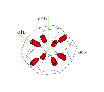
\includegraphics[width=0.4\textwidth]{valleys.eps}  
  \caption{Orientations of the crystal axes and valleys in the lab coordinate system XYZ.}
  \label{fig:valley}
\end{figure}

The dependence of the electron drift velocity $\mathbf{v}_{e}$ on the applied electric field $\mathbf{E}$ is taken to be
\begin{equation}
  \label{eq:ed}
  \mathbf{v}_{e}(\mathbf{E}) = \mathcal{A}(|\mathbf{E}|) \sum_{j} \frac{n_{j}}{n}     \frac{\gamma_{j}\mathbf{E_{0}}}     {\sqrt{\mathbf{E_{0}}\gamma_{j}\mathbf{E_{0}}}},  \mbox{ with }     j=1,2,3,4
\end{equation}
where $\mathcal{A}$ is a function of the magnitude of the electric field and temperature, the value of $\mathcal{A}$ must be negative because electrons drift to the opposite direction of the electric field; $\mathbf{E_{0}}$ is the normalized electric field vector; $n_{j}/n$ is the fraction  of the carriers (in this case, electrons) in the $j$-th valley, $\gamma_{j}$ is the effective mass tensor for the $j$-th valley. In general the tensor $j$-th is given in terms of the rotation matrices $R_{i}$, responsible for aligning the $i$-th $\langle 111 \rangle$ axis with the Y-axis of the lab system, by
\begin{equation}
  \label{eq:gammas}
  \gamma_{j} = R_{j}^{T}\gamma_{0}R_{j}, \mbox{ with } \gamma_{0}   \equiv \left(
    \begin{array}{ccc}
      m_{t}^{-1} & 0 & 0 \\
      0 & m_{l}^{-1} & 0 \\
      0 & 0 & m_{t}^{-1}
    \end{array} \right),
\end{equation}
where $m_{t} = 1.64m_{e}, m_{l} = 0.0819m_{e}$ with $m_{e}$ denoting the free electron mass, and the rotation matrix $R_{j} = R_{x^{\prime}}(\arccos(\sqrt{2/3}))R_{z}((j-1)\pi/2)$.

\begin{figure}[tbhp]
  \centering
  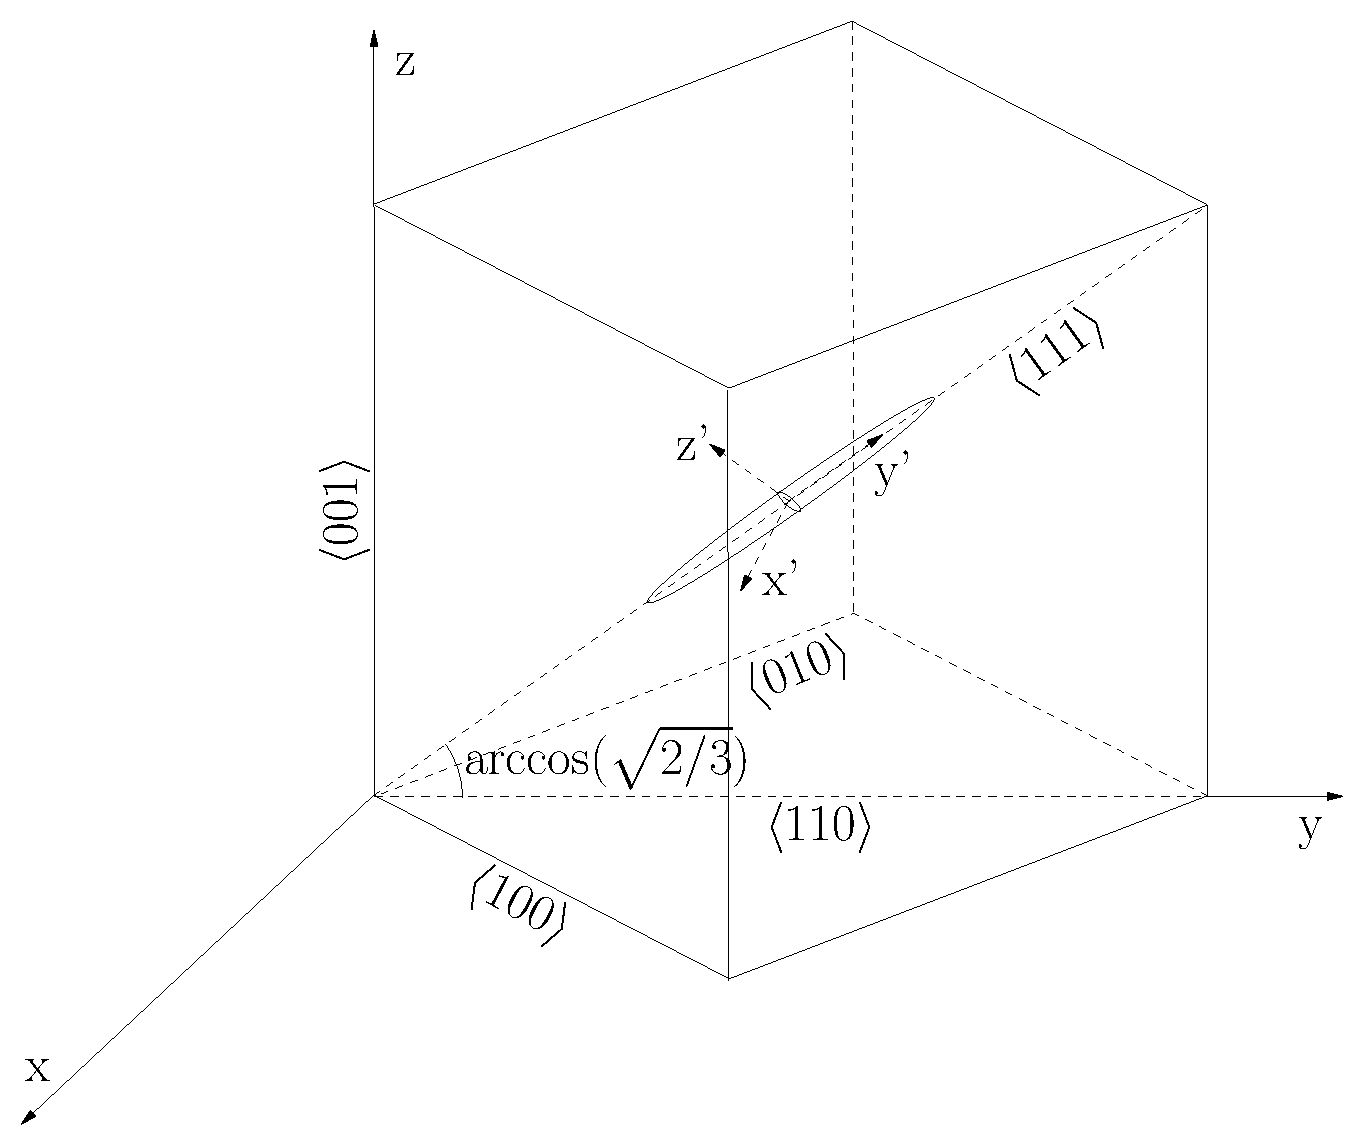
\includegraphics[width=0.6\textwidth]{axes.eps}  
  \caption{Orientations of the crystal axes and valleys in the lab coordinate system XYZ.}
  \label{fig:axes}
\end{figure}

For an experimental determination of the repopulation amplitude, the deviation from a uniform population distribution $n_{e}/n$ (1/4 for germanium) is assumed to vary with the electric field weighted by the factor $\mathcal{R}$:
\begin{equation}
  \label{eq:nion}
  \frac{n_{j}}{n} = \mathcal{R(|\mathbf{E}|)}   \left[         \frac{\sqrt{\mathbf{E_{0}}\gamma_{j}\mathbf{E_{0}}}}
    {\sum_{i}\sqrt{\mathbf{E_{0}}\gamma_{i}\mathbf{E_{0}}}} -               \frac{n_{e}}{n} \right] + \frac{n_{e}}{n},  \mbox{ with }           i=1,2,3,4
\end{equation}

If the electric field vector is equally oriented with respect to all the $\langle111\rangle$ directions, there is an uniform repopulation of the conduction bands, \textit{i.e.} $n_{j}/n = 1/4$. An electric field applied along the $\langle100\rangle$ direction, \textit{i.e.} $\mathbf{E_{0}} = (1/\sqrt{2},1/\sqrt{2},0)^{T}$, satisfies this condition. By employing the experimental drift velocity $v_{e}^{exp}(E)$ for an applied electric field $E$ in the $\langle100\rangle$ direction at a specific temperature, the absolute value  of $\mathcal{A}(|\mathbf{E}|)$ can be calculated as
\begin{equation}
  \label{eq:ae}
  \mathcal{A}(|\mathbf{E}|) = \frac{v_{e}^{exp}(E)}  {\displaystyle \sum_{j}     \frac{1}{4}     \frac{\gamma_{j}\mathbf{E_{0}}}         {\sqrt{\mathbf{E_{0}}\gamma_{j}\mathbf{E_{0}}}} },  \mbox{ with }       \mathbf{E_{0}} = \left( \begin{array}{c} 
    1/\sqrt{2}\\1/\sqrt{2}\\0 \end{array} \right).
\end{equation}

If the electric field vector is oriented along with one of the $\langle111\rangle$ directions, \textit{i.e.} $\mathbf{E_{0}} = (0,\sqrt{2}/\sqrt{3},1/\sqrt{3})^{T}$, there is an uniform repopulation of the conduction bands among the other three $\langle111\rangle$-axes, \textit{i.e.}
\begin{equation}
  \label{eq:n111}
  \frac{n_{2}}{n} = \frac{n_{3}}{n} = \frac{n_{4}}{n}.
\end{equation}
Since
\begin{equation}
  \label{eq:nsum}
  \displaystyle \sum_{j}\frac{n_{j}}{n} = 1,
\end{equation}
we have
\begin{equation}
  \label{eq:n12}
  \frac{n_{1}}{n} + 3\frac{n_{2}}{n}= 1.
\end{equation}
By employing the experimental drift velocity $v_{e}^{exp}(E)$ for an applied electric field $E$ in the $\langle111\rangle$ direction at a specific temperature, we have another relation between $n_{1}/n$ and $n_{2}/n$:
\begin{equation}
  \label{eq:n12p}
  v_{e}^{exp}(E) =  \mathcal{A}(|\mathbf{E}|) \left(  \frac{n_{1}}{n} \frac{\gamma_{1}\mathbf{E_{0}}}         {\sqrt{\mathbf{E_{0}}\gamma_{1}\mathbf{E_{0}}}} +  3\frac{n_{2}}{n} \frac{\gamma_{2}\mathbf{E_{0}}}         {\sqrt{\mathbf{E_{0}}\gamma_{2}\mathbf{E_{0}}}} \right).
\end{equation}
One can get the value of $n_{1}/n$ and $n_{2}/n$ by solving the equations \ref{eq:n12} and \ref{eq:n12p} together. Then $\mathcal{R}(|\mathbf{E}|)$ can be calculated as
\begin{equation}
  \label{eq:re}
  \mathcal{R(|\mathbf{E}|)} = \left( \frac{n_{1}}{n} - \frac{n_{e}}{n}     \right) / \left(     \frac{\sqrt{\mathbf{E_{0}}\gamma_{1}\mathbf{E_{0}}}}
    {\sum_{i}\sqrt{\mathbf{E_{0}}\gamma_{i}\mathbf{E_{0}}}} -                           \frac{n_{e}}{n} \right),  \mbox{ with }           i=1,2,3,4 \mbox{ and       } \mathbf{E_{0}} = \left( \begin{array}{c} 
      0\\ \sqrt{2}/\sqrt{3}\\1/\sqrt{3} \end{array} \right).
\end{equation}

The dependence of the experimental $\langle111\rangle$ and $\langle100\rangle$ drift velocities on the electric field can be fitted with the empirical formula: 
\begin{equation}
  \label{eq:expe}  
  v_{e}^{exp}(E) = \frac{\mu_{0}E}{(1+(E/E_{0})^{\beta})^{1/\beta}} - \mu_{n}E.
\end{equation}
The fitted parameters values are presented in Table~\ref{tab:pars}
\begin{table}[tbhp]
  \centering
  \begin{tabular}{ccccc}\hline\hline
    Direction & $\mu_{0} \left[ \frac{\mbox{cm}^{2}}{\mbox{V}\cdot\mbox{s}} \right]$ & $E_{0} \left[ \frac{\mbox{V}}{\mbox{cm}} \right]$ & $\beta$ & $\mu_{n} \left[ \frac{\mbox{cm}^{2}}{\mbox{V}\cdot\mbox{s}} \right]$ \\\hline
$\langle111\rangle$ & 40180 & 493 & 0.72 & 589 \\
$\langle100\rangle$ & 42420 & 251 & 0.87 & 62\\ \hline\hline
  \end{tabular}
  \caption{Fit parameters for the experimental drift velocities in the 
$\langle111\rangle$ and $\langle100\rangle$ directions.}
\label{tab:pars}
\end{table}

After determination of the parameters $\mathcal{A}$ and $\mathcal{R}$, the drift velocity can be calculated for any direction and any strength of the electric field.

\subsection{Hole Drifting}
\label{sec:hole}
\begin{equation}
  \label{eq:vsphere}
  \begin{array}{rcl}
   v_{r} &=& v_{100}(E)[1-\Lambda(k_{0})(\sin(\theta)^{4}\sin(2\phi)^{2} + \sin(2\theta)^{2})]\\
   v_{\theta} &=& v_{100}(E)\Omega(k_{0})[2\sin(\theta)^{3}\cos(\theta)\sin(2\phi)^{2} + \sin(4\theta)]\\
    v_{\phi} &=& v_{100}(E)\Omega(k_{0})\sin(\theta)^{3}\sin(4\phi)
  \end{array}
\end{equation}


\begin{figure}[tbhp]
  \centering
  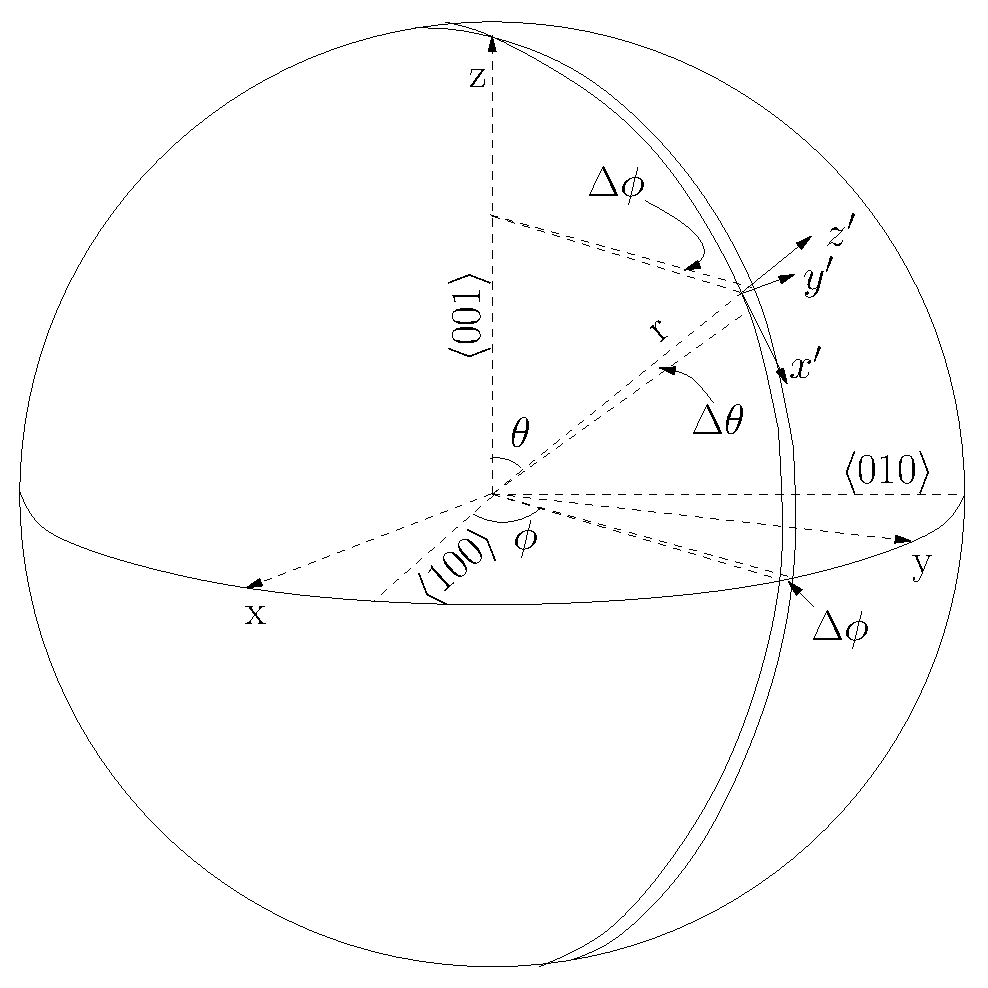
\includegraphics[width=0.5\textwidth]{vsphere.eps}  
  \caption{Orientations of the crystal axes and valleys in the lab coordinate system XYZ.}
  \label{fig:vsphere}
\end{figure}


%%% Local Variables:
%%% mode:latex
%%% TeX-master: "GSTR-08-M00x"
%%% End:

\subsection{Formation of detector signals}
\label{sec:signal}




%%% Local Variables:
%%% mode:latex
%%% TeX-master: "GSTR-08-M007"
%%% End:


\section{Verification of the simulation}
\label{sec:verify}

\subsection{Electric and weighting fields}
\label{subsec:efield_wfield}
The radial component of the electric field of a true coaxial germanium crystal can be calculated analytically 
\begin{equation}
  \label{eq:EFieldAnalytical}
  |E(r)| = \frac{eN_{A}}{2\epsilon_{0}\epsilon_{R}} r + \frac{V - (eN_{A}/4\epsilon_{0}\epsilon{R})(r_{2}^{2}-r_{1}^{2})}{r \ln(r_{2}/r_{1})},
\end{equation}
with inner and outer radii $r_1$ and $r_2$ and $V = \varphi(r_2) - \varphi(r_1)$. The other components $E(\varphi,z)$ could be calculated analytically, but they are zero.
The weighting potential and field of the segments cannot be calculated analytically, but the numerical method to calculated the electric field and the weighting fields are the same. By comparing the results of the numerical calculation of the electric field and the analytical one, one gains trust into the calculation of the weighting fields.


The result of the analytic and numeric calculation of the electric field for a 18 fold segmented true coaxial n-type germanium detector are shown in \figref{fig:efields}. The simulated detector has a inner radius of $r_{1} = 0.005$~m and an outer radius $r_{2} = 0.0375$~m. The height is $0.07$~m. The simulated applied voltage is $3000$~V on the core. The charge carrier density is $0.68\cdot 10^{10} \text{~cm}^{-3}$, which corresponds to a depletion voltage of $2500$~V. The numerical calculation was done on a $100 \ast 100 \ast 100$ grid and the calculation was stoped at a relative overall change of $1 \cdot10^{-6}$. 
%%%%%%%%
%%Figure: EFields
%%%%%%%%
\begin{figure}[tbhp]
  \centering
  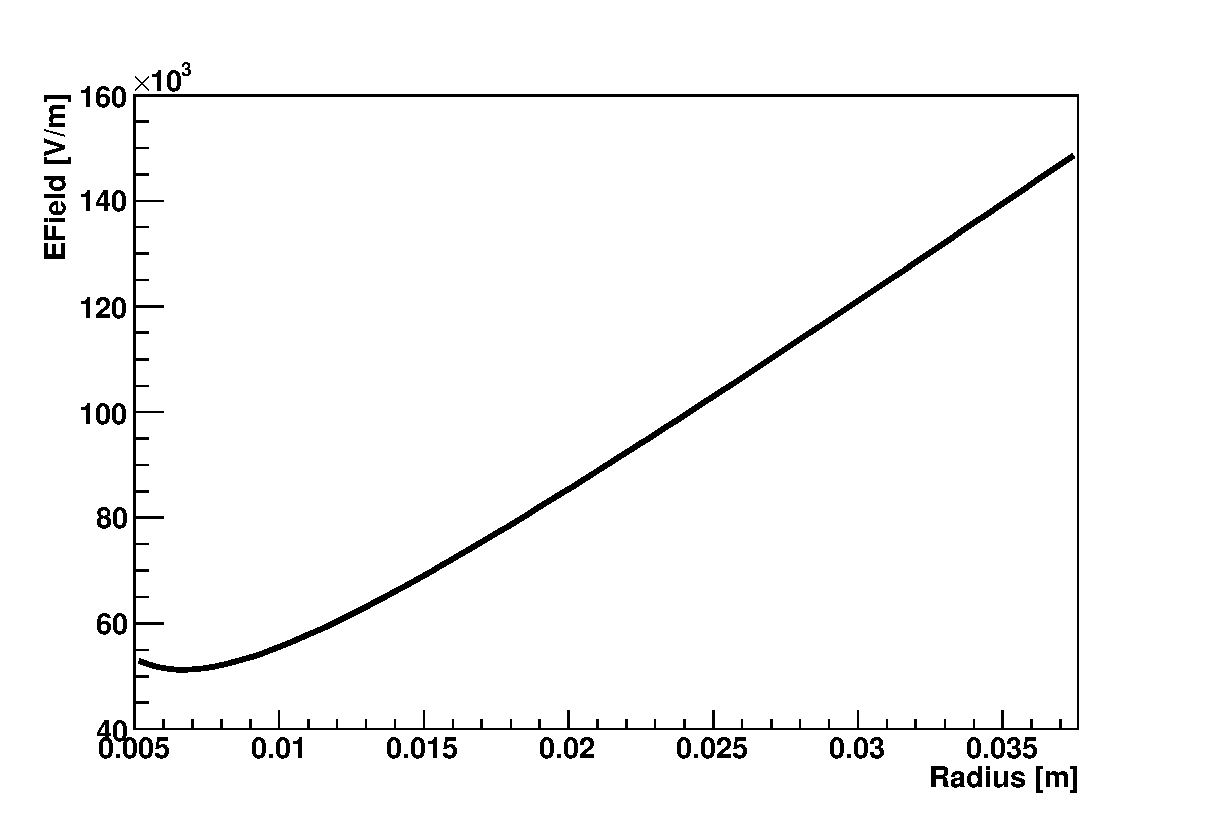
\includegraphics[width=0.49\textwidth]{EFieldAnalytical.eps}
  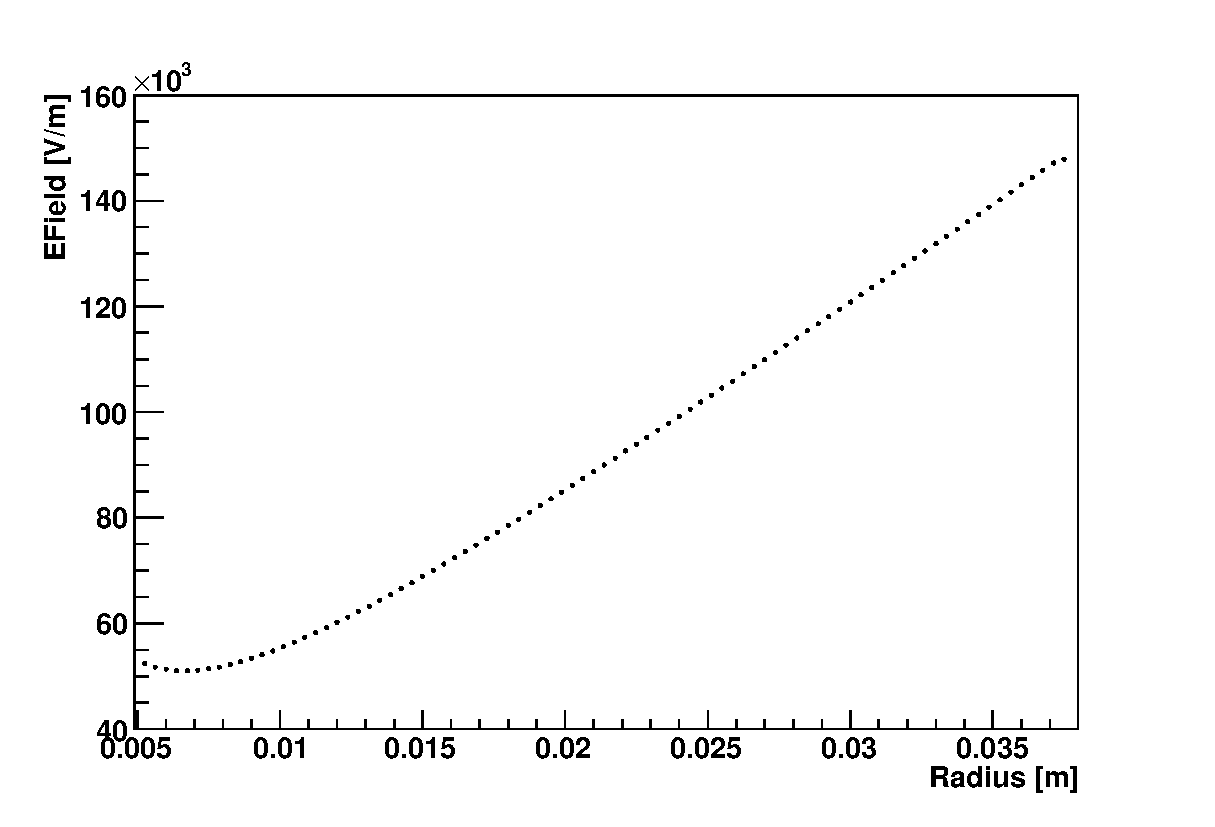
\includegraphics[width=0.49\textwidth]{EFieldNum.eps}
  \caption{Electric field as a function of radius r. (\emph{left}) Electric field from an analytical calculation according to \eqref{eq:EFieldAnalytical}. (\emph{right}) Electric field from a numerical calculation according to the method described in Sec.\,\ref{sec:field}. }
  \label{fig:efields}
\end{figure}
%%%%%%%%%%%%%%%

The relative difference of the electric field from the analytical and numerical calculation is shown in \figref{fig:efieldsRelDifference} as a function of the radius. The biggest deviation from the exact solution is of the order of $0.6$~\%.
%%%%%%%%
%%Figure: relative difference
%%%%%%%%
\begin{figure}[tbhp]
  \centering
  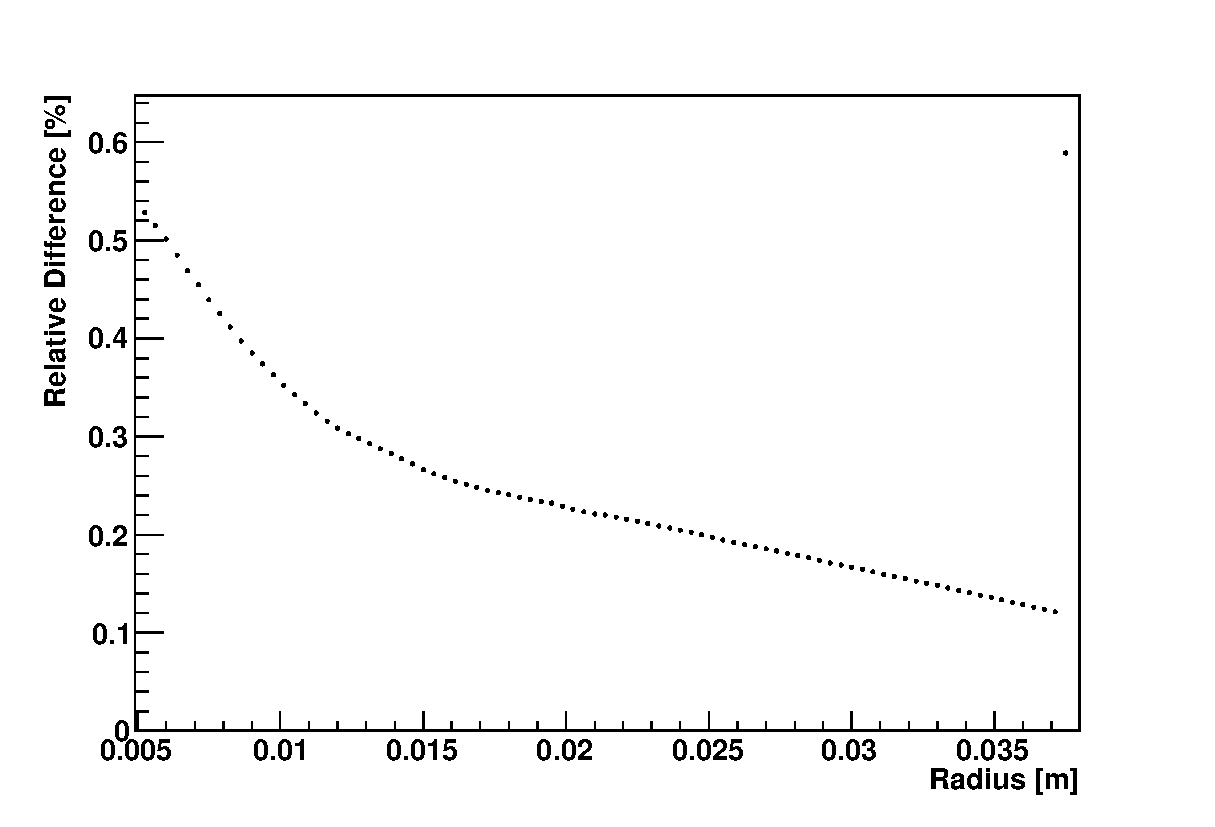
\includegraphics[width=0.8\textwidth]{relativeDifference_Num-Analyt.eps}
  \caption{Relative difference in \% in the electric fields from analytical to numerical calculation.}
  \label{fig:efieldsRelDifference}
\end{figure}
%%%%%%%%%%%%%%

%%% Local Variables:
%%% mode:latex
%%% TeX-master: "GSTR-08-M007"
%%% End:

\subsection{Charge carrier drift}
\label{subsec:drift}
Some control plots are made in order to check whether the simulation of the charge carrier drifts makes sense or not. The crystal implemented in the simulation is a GERDA phase II prototype detector~\cite{Siegfried}. It is made of a true coaxial cylindrical natural germanium crystal. The applied high voltage is 3000~V.

\subsection{Longitudinal anisotropy}
\label{subsec:long}
Figure~\ref{fig:vvse} shows the drift velocities along crystal axes as functions of electric field in [7,500]~V/mm. There is no transverse anisotropy of the drift along crystal axes. This figure is used to show the longitudinal difference of the drift velocity in different directions. 
\begin{figure}[tbhp]
  \centering
  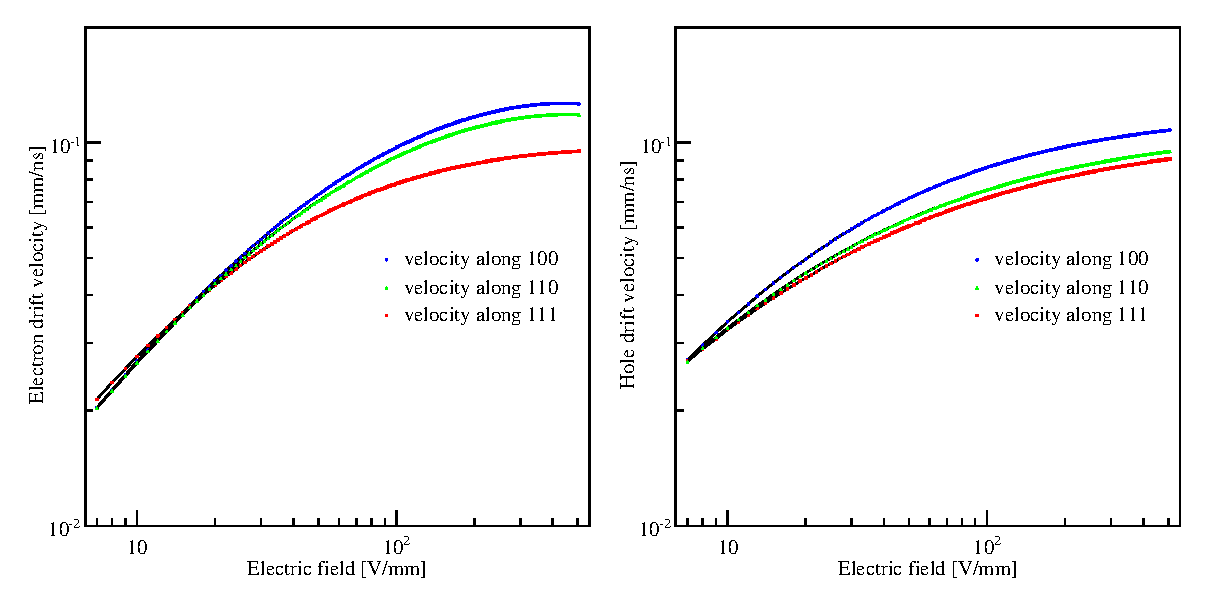
\includegraphics[width=1.0\textwidth]{VvsElucian} \\\hfil
  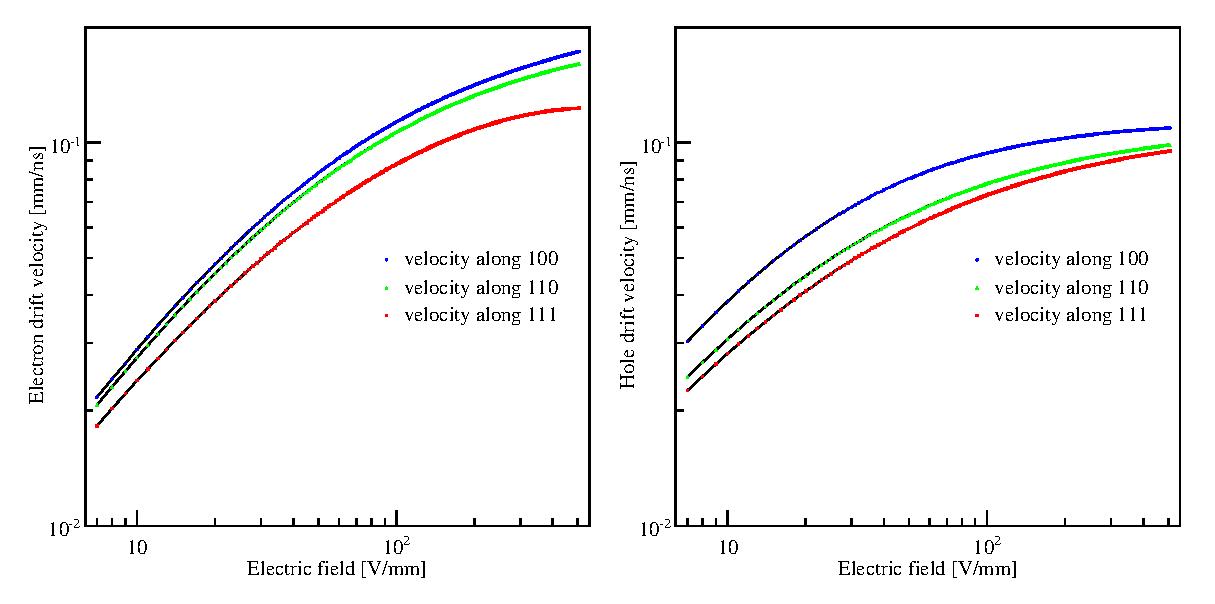
\includegraphics[width=1.0\textwidth]{VvsEbart}
  \caption{Drift velocities along crystal axes as functions of electric field in [7,500]~V/mm. Velocities along crystal axes $\langle 100 \rangle$ and $\langle 111 \rangle$ are calculated with eq.~\ref{eq:para}, while velocities along $\langle 110 \rangle$ are the simulated results. The upper plots are created using the input parameters provided in Ref.~\cite{miha}, the lower using the input parameters provided in Ref.~\cite{bart}.}
  \label{fig:vvse}
\end{figure}

\subsection{Transverse anisotropy}
\label{subsec:long}
Figure~\ref{fig:trjs} shows the charge carrier drift trajectories on X-Y plane. The transverse anisotropy causes the bend of the trajectories. Also shown are the cross section of a true coaxial cylindrical germanium detector with inner radius of 5~mm and outer radius of 37.5~mm. The crystal axes are indicated with the signs $\langle 100 \rangle$, $\langle 110 \rangle$ and $\langle 010 \rangle$. The left plot shows the drift of electrons starting from the outer surface of the detector to the inside. The start points are distributed along the outer circle with equal distance between each other. The right plot shows the drift of holes starting from the inner surface to the outside. The start points are distributed along the inner circle with equal distance between each other. The applied high voltage is 3000~V. The time window is 400~ns. Within this time window all the electrons could reach the inner circle, while not all the holes could reach the outer circle.  This is because electrons drift slightly faster than holes, and along $\langle 110 \rangle$ direction holes drift slowest, as shown also in Fig.~\ref{fig:vvse}.
\begin{figure}[tbhp]
  \centering
  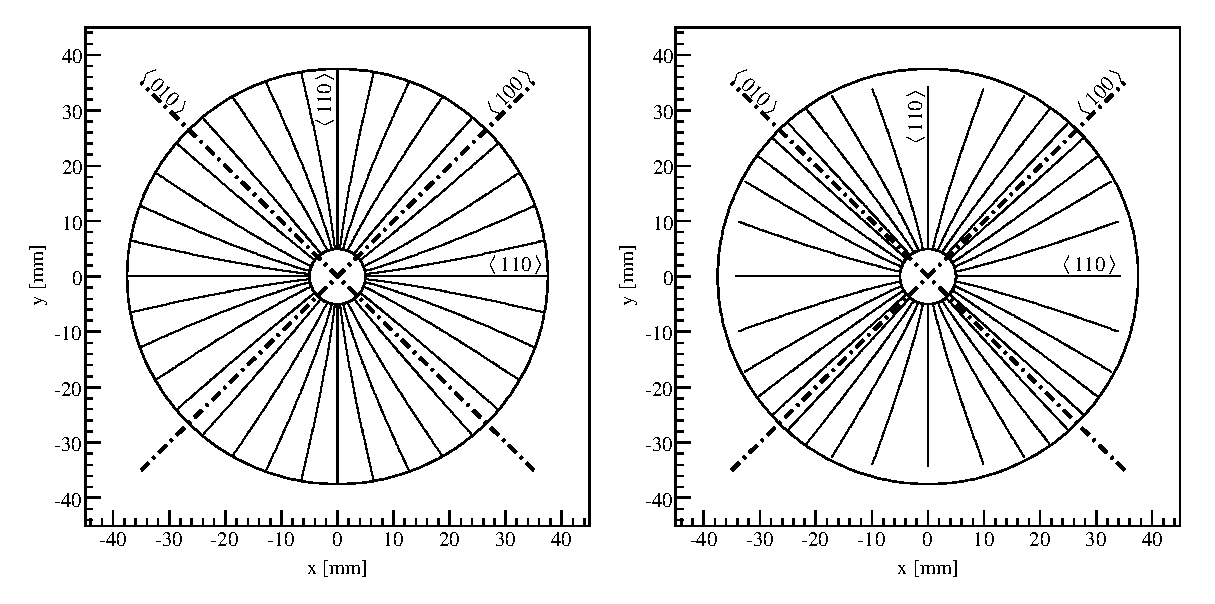
\includegraphics[width=1.0\textwidth]{trjs}
  \caption{Charge carrier drift trajectories on X-Y plane. The     transverse anisotropy causes the bend of the trajectories. Also     shown are the cross section of a true coaxial cylindrical     germanium detector with inner radius of 5~mm and outer radius of     37.5~mm. The crystal axes are indicated with the signs $\langle     100 \rangle$, $\langle 110 \rangle$ and $\langle 010 \rangle$. The     left plot shows the drift of electrons starting from the outer     surface of the detector to the inside. The start points are     distributed along the outer circle with equal distance between     each other. The right plot shows the drift of holes starting from     the inner surface to the outside. The start points are distributed     along the inner circle with equal distance between each other. The     applied high voltage is 3000~V. The time window is 400~ns. Within     this time window all the electrons could reach the inner circle,     while not all the holes could reach the outer circle. This is     because electrons drift slightly faster than holes, and along     $\langle 110 \rangle$ direction holes drift slowest, as shown also     in Fig.~\ref{fig:vvse}.}
  \label{fig:trjs}
\end{figure}


%%% Local Variables:
%%% mode:latex
%%% TeX-master: "GSTR-08-M007"
%%% End:


\section{Pulse shape analysis}
\label{sec:physics}


\clearpage
 
\addcontentsline{toc}{section}{Bibliography}
\begin{thebibliography}{99}
\bibitem{gerda} I. Abt \textit{et al.}, Letter of Intent for GERDA   Experiment, hep-ex/0404039.
\bibitem{comcon} B. Aspacher, A. C.  Rester, Nucl. Instr. and Meth.   in Phys. Res. A \textbf{338} (1994) 511.
\bibitem{agata}J. Gerl, W. Korten eds., Online AGATA Technical   Proposal, http://agata.pd.infn.it/documents/Agata-proposal.pdf   (2001).
\bibitem{major} S. R. Elliott \textit{et al.}, Nucl. Instr. and   Meth. in Phys. Res. A \textbf{558} (2006) 504.
\bibitem{xiang} I. Abt \textit{et al.}, Eur. Phys. J. C \textbf{54}   (2008) 425.
\bibitem{mage} Yuen-Dat Chan \textit{et al.}, arXiv:nucl-ex/0802.0860.
\bibitem{igex} D. Gonz\'alez \textit{et al.}, Nucl. Instr. and Meth.   in Phys. Res. A \textbf{515} (2003) 634.
\end{thebibliography}

%%% Local Variables:
%%% mode:latex
%%% TeX-master: "GSTR-08-M007"
%%% End:


\end{document}

